\section{Requirements}
\label{requirement}

\subsection{Preliminary Analysis}
We first performed analysis on the given proposal in Section \ref{scope}. On the infrastructure side, the proposal requires the project to be integrated into Jira. Among the different versions of Jira software available, the team chose Jira Cloud over Jira Server, for its cloud-based nature is more compatible in modern workplace. 

For the purpose of our project, we consider the following key concepts. 
\textbf{Epic} is defined as a collection or narrative of user stories; they contain more information as to the functional usage of a target project being documented. The next level is \textbf{User Story}, which is a compact set of requirements. These requirements can be further broken down into \textbf{Tasks}, actionable items to be completed as part of a user story. 
Epic, User Story, and Tasks are the three levels of requirements items that our tool focuses on. 

\subsection{Requirement Modeling with KAOS}
First, the team modeled the requirements using KAOS models\cite{KAOS}. KAOS is a Goal-oriented requirement engineering \cite{GOAL} tool that emphasizes goals in requirement acquisition. The team built the KAOS models to guarantee thorough traceability across all requirements, which includes describing the problems, identifying top level goals to address problems and stating the constraint for solutions, etc. Moreover, using the KAOS models, the team could easily remove or add requirements as we encounter new information and changes. The KAOS tutorial handbook \cite{KAOS} also provides universally applicable generic patterns for reference, and we specified our initial goals by adopting these patterns, with selected models presented below.

\begin{figure}
\centering
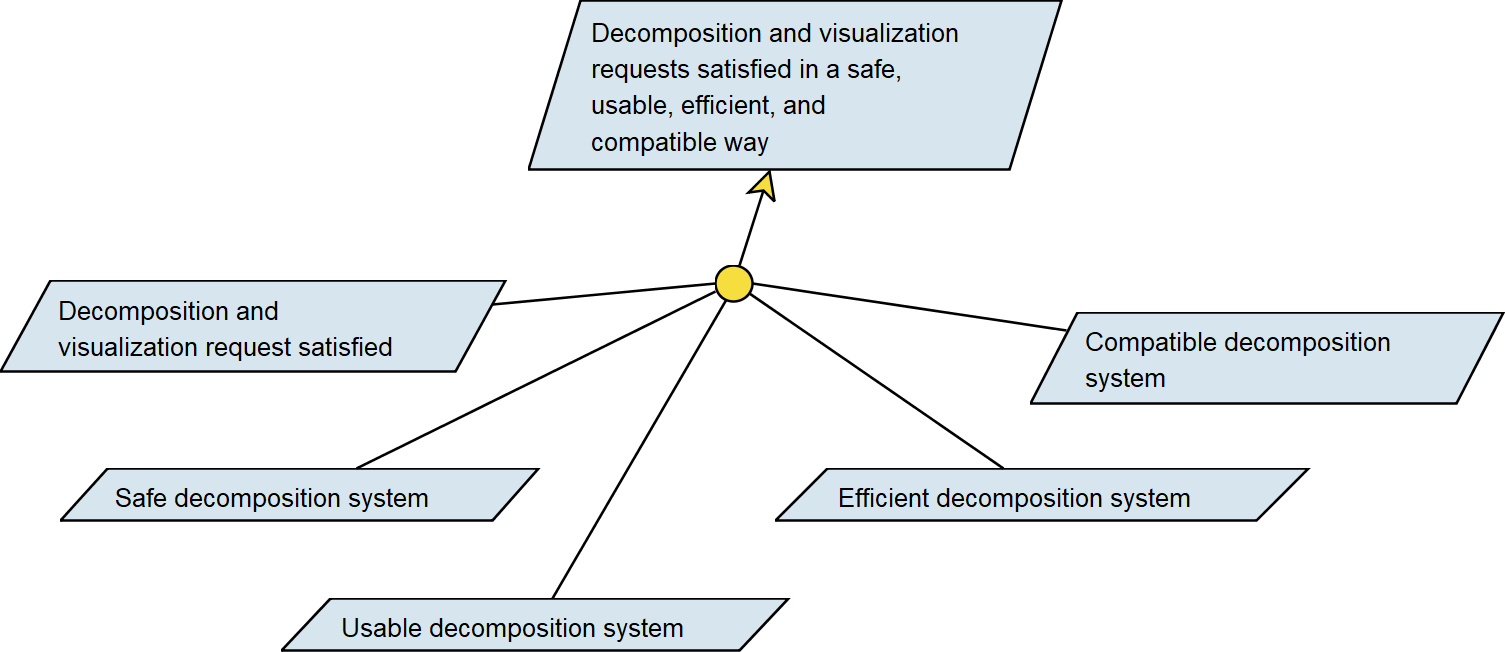
\includegraphics[width=\textwidth,keepaspectratio]{./figure/GoalsNFR1.png}
\caption{Top level goal model of AI4Agile}
\label{goal1}
\end{figure}

We identify three primary processes to handle the requirements items defined above: 1) Epic Decomposition, 2) Story Optimization, and 3) Task Generation. Fig. \ref{goal1} defines the top-level goal for the entire system, with subgoals that enumerate all cases that must be covered to fulfill our main goal. The subgoals each encompasses a portion of the functional and nonfunctional requirements (FRs and NFRs) of the system. As shown in Fig. \ref{goal1}, the goals that our system should achieve are:

\begin{itemize}
	\item Decomposition and visualization request satisfied
	\item Safe decomposition system
	\item Usable decomposition system
	\item Efficient decomposition system
	\item Compatible decomposition system
\end{itemize}

The goals for “Safe”, “Usable”, “Efficient”, and “Compatible System” covered the NFR portion of the system. By using respective generic patterns from \cite{KAOS}, we generated the nonfunctional requirements for our system as shown in Table \ref{nfrs}.

\begin{table}
\centering
\caption{Non-functional requirements}
\label{nfrs}
\begin{tabular}{ |c|c| } 
\hline
\multicolumn{1}{|c|}{\textbf{ID}} & \multicolumn{1}{c|}{\textbf{Description}} \\
\hline
NFR1 & Show resources about Agile development \\
\hline
NFR2 & Follow Agile development process \\
\hline
NFR3 & Have presets for user without domain expertise \\
\hline
NFR4 & Show notification about decomposition status \\
\hline
NFR5 & Do not store information on third-party database \\
\hline
NFR6 & Only query Jira the information that is needed \\
\hline
NFR7 & Software is secure \\
\hline
NFR8 & Retain original sentences in epics with minimal modification \\
\hline
NFR9 & The response time for AI processing is less than five seconds \\
\hline
NFR10 & The response time for visualization is less than two seconds \\
\hline
NFR11 & Visualization only generates important relationships \\
\hline
NFR12 & Available on Atlassian Marketplace \\
\hline
NFR13 & Available on Atlassian Partner Marketplace \\
\hline
\end{tabular}
\end{table}

\begin{figure}
\centering
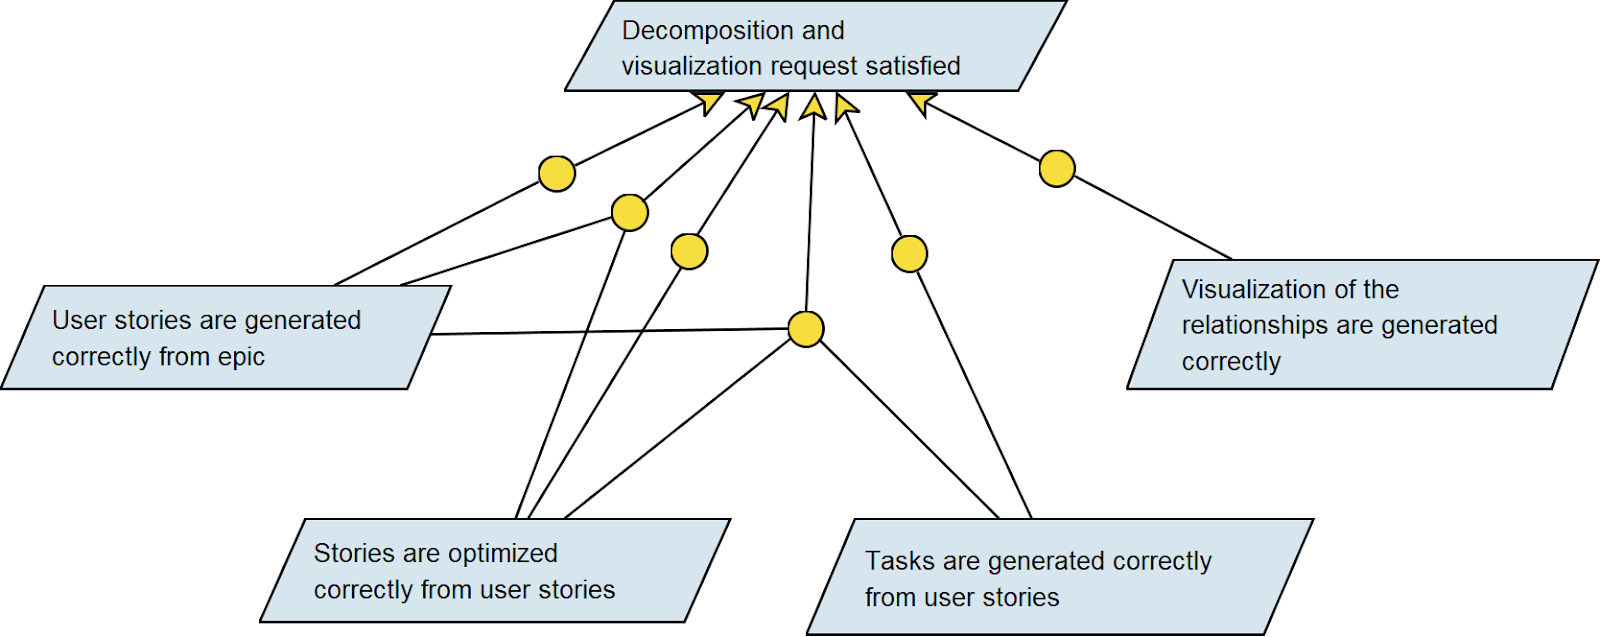
\includegraphics[width=\textwidth,keepaspectratio]{./figure/GoalsNFR2.png}
\caption{Functional goal decomposition continued from Fig. \ref{goal1}}
\label{frgs}
\end{figure}

Next, we broke down the “decomposition request and visualizations satisfied” goal into subgoals, which correlated to the main FRs. Fig. \ref{frgs} shows the first level of functional subgoals, listed below: 

\begin{itemize}
	\item User stories are generated correctly from epic
	\item Stories are optimized correctly from user stories
	\item Tasks are generated correctly from user stories
	\item Visualization of the relationships are generated correctly
\end{itemize}

Each subgoal in Fig. \ref{frgs} has its own KAOS goal models that were further refined. Due to space constraint, we include one example in Fig. \ref{fr1}. Fig \ref{fr1} shows how we refined the subgoal ``User stories are generated correctly from epic'' into the specification. It also identifies the agents responsible for fulfilling this subgoal.  From these models, we obtained the functional requirements as shown in Table \ref{frt}.

\begin{figure}
\centering
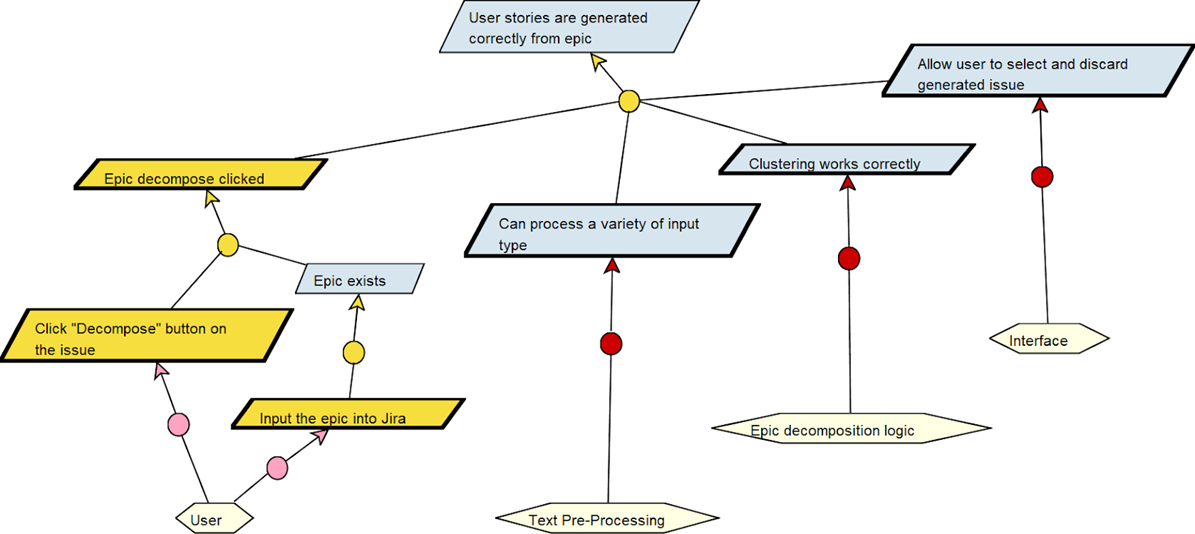
\includegraphics[width=\textwidth]{./figure/GoalsFR1.png}
\caption{Further refinement of one subgoal in Fig. \ref{frgs}}
\label{fr1}
\end{figure}

\begin{table}
\centering
\caption{Functional requirements}
\label{frt}
\begin{tabular}{ |c|c| } 
\hline
\multicolumn{1}{|c|}{\textbf{ID}} & \multicolumn{1}{c|}{\textbf{Description}} \\
\hline
FR1 & Clustering works correctly \\
\hline
FR2 & Allow user to select and discard generated issue \\
\hline
FR3 & Can process a variety of input types \\
\hline
FR4 & User stories extraction works correctly \\
\hline
FR5 & Retain user stories if those are small enough \\
\hline
FR6 & Sentence building works correctly \\
\hline
FR7 & Show the explicit relationship between issues as a tree \\
\hline
FR8 & Show the implicit relationship of developers to the issues as clusters \\
\hline
FR9 & Allow user to show and edit relationship \\
\hline
FR10 & Show a customizable type and depth to relationship between issues \\
\hline
FR11 & The graph should render as the object is selected \\
\hline
\end{tabular}
\end{table}

\subsection{Requirements Summary}
The NFRs and FRs in Tables \ref{nfrs} and \ref{frt} defined the initial scope for our implementation, each with their own specifications developed. To summarize the system's three major functional processes, we concluded that: 1) Epic decomposition means that, given a semi-structured, manually entered epic, the app would refine it into user stories in the form of subject-based clusters; 2) Story optimization further breaks down large stories into smaller stories; 3) Task generation is done by performing part-of-speech analysis on the user stories. 

Furthermore, to satisfy the NFRs such as integrity, for each process, the app would offer suggestion results to the user, allowing them to pick and choose which user stories and tasks to add to their Jira board. The user can further adjust settings, i.e. number of tasks to be generated, to fine tune the granularity of generated results. Finally, epics, user stories, and tasks can be displayed in an interactive tree/cluster graph that shows the explicit and implicit relationships among them.

The project's main motivation is to save time for manual Requirement Engineering (RE). While AI could be used in different ways to achieve this goal, our app predominantly utilized the AI component in text processing, generating increasingly refined results to support an efficient RE process. This approach could also increase the consistency of the RE outcomes, as the central process reduces the impact of human factors. In the meantime, we recognized that knowledge and experiences from a skilled project manager is still crucial, thus we make sure that the tool would not alter or discard any original input, preventing unintended consequences. Last but not least, with direct feedback from our mentor, the team formatted sample requirements we have encountered in practice, and developed the user stories used for demo and verification purposes, as presented in Section \ref{demo}.